\section{Methodology}
Once we have configured the schema \& defined the ontology, our KG construction pipeline comprises of four interlocking components: (1) Intelligent Document Parsing Layer, (2) Table-Aware Semantic Chunking Layer, (3) Iterative Prompt \& Agent Driven Triples Extraction Layer, and (4) Robust Evaluation Layer. By integrating best practices from AI-driven information extraction and financial KG construction, we achieve both high precision and domain relevance. The overall pipeline is showcased in the Figure~\ref{fig:graph_rag_microservice}

\begin{figure}[htbp]
    \centering
    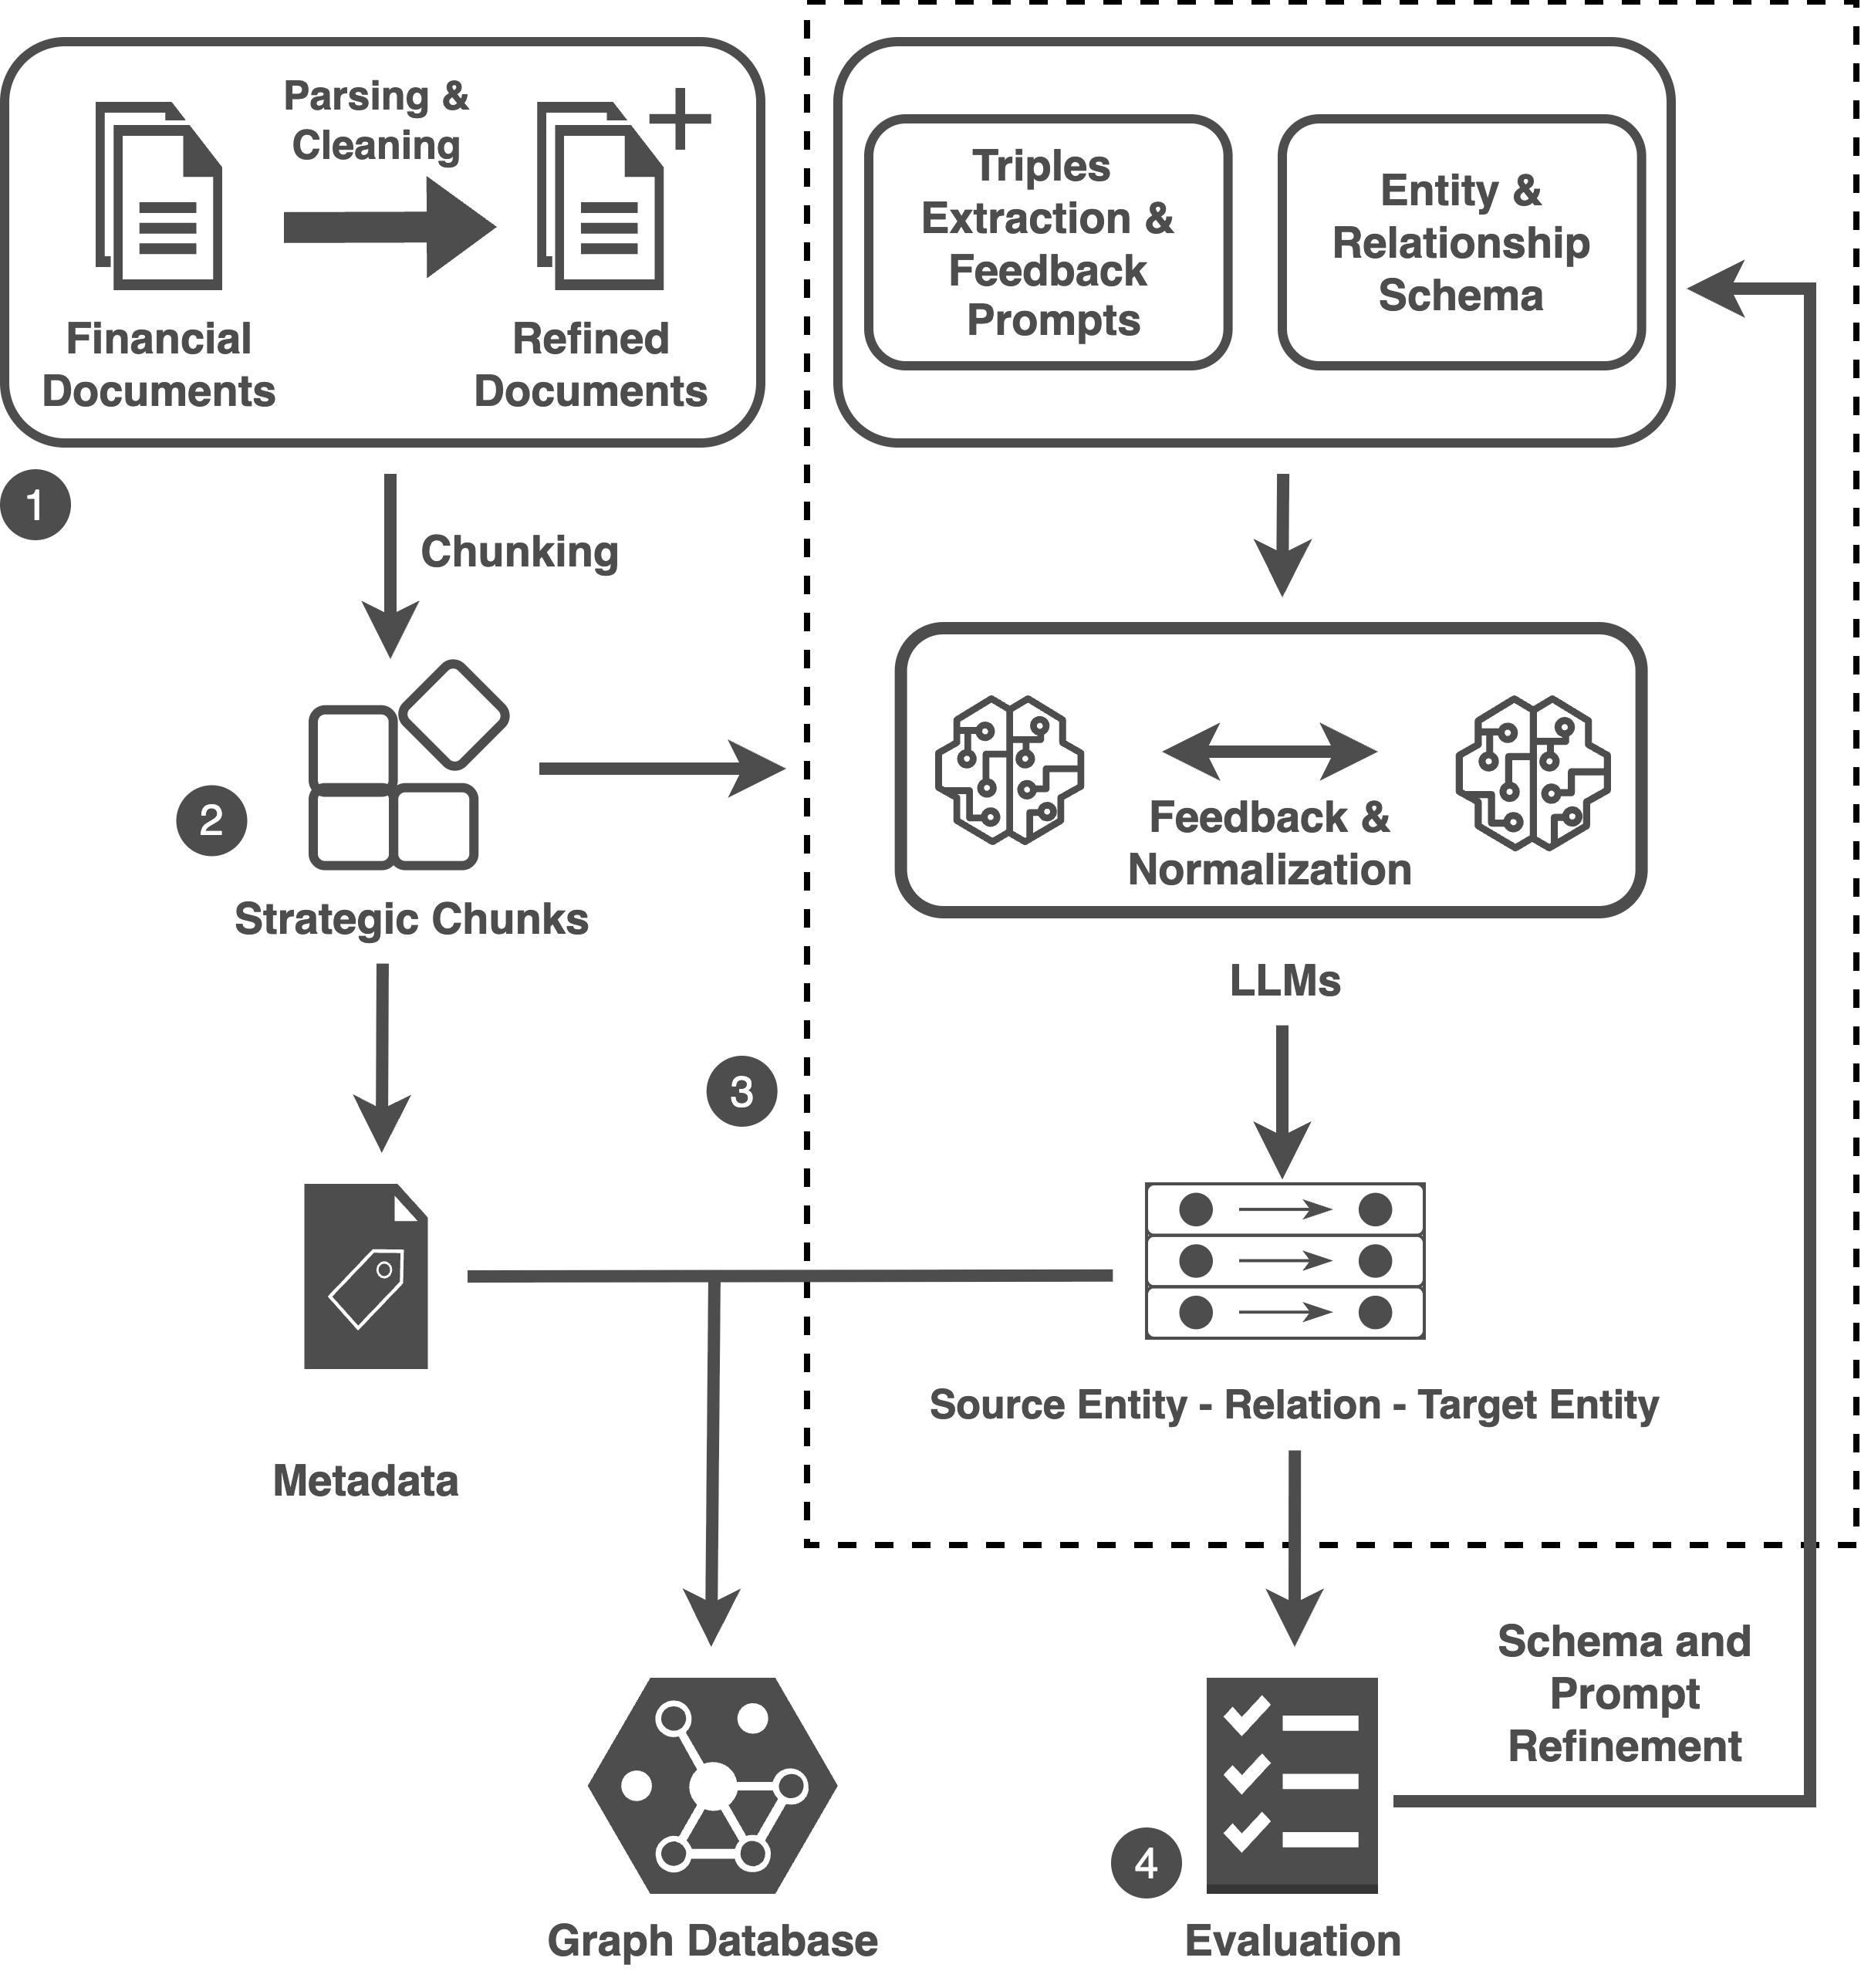
\includegraphics[width=\columnwidth]{figures/kg_pipeline_diagram.png}
    \caption{Overview of the Graph RAG microservice and its integration with the KG construction pipeline.}
    \label{fig:graph_rag_microservice}
\end{figure}
\subsection{Intelligent Document Parsing Layer}

Our pipeline leverages an advanced document parsing layer built on \texttt{docling} \cite{auer2024docling}, enabling robust extraction and retention of the diverse formats present in SEC 10-K filings. This layer preserves the multiformat architecture of the source documents, including narrative text, tables, and images. Tables are especially critical in financial filings, as they often encapsulate key quantitative disclosures (e.g., revenue by segment, risk breakdowns, or financial metrics) essential for downstream knowledge graph construction.

The parser operates in two modes: a \textbf{multimodal mode}, which combines OCR and image annotation to capture both textual and visual information, and a \textbf{text-only mode} for efficient processing when only narrative content is required. For the scope of this paper, we used only the text mode. In both modes, tables structures are retained as markdown context, maintaining row–column associations and semantic context. Narrative sections are tagged with section headers (e.g., ``Risk Factors,'' ``Management's Discussion'') to facilitate schema alignment in subsequent pipeline stages.

This intelligent parsing approach ensures that no critical information is lost during preprocessing, and provides a high-fidelity, semantically annotated representation of the original document for downstream chunking and extraction.

\subsection{Table-Aware Semantic Chunking Layer}

To accommodate the token limits of modern large language models, our pipeline incorporates a custom chunking algorithm that strategically segments documents while preserving semantic and structural integrity. Unlike naive sliding window or fixed-length approaches, our chunker is \textbf{table-aware}: any detected table in the markdown is retained as a single atomic chunk, ensuring that row and column relationships—and thus the full context of financial data—are never fragmented. This is particularly important for SEC 10-K filings, where tables often encode critical quantitative disclosures.

We employ a \textbf{section-aware text segmentation}, splitting text at logical boundaries such as paragraphs or subsection headings to maintain topical coherence. Each chunk is constrained to a maximum size of 2048 tokens (\texttt{CHUNK\_SIZE = 2048}), balancing context preservation with LLM input requirements.

This approach ensures that both tabular and textual information are optimally prepared for downstream extraction, maximizing the fidelity and relevance of the knowledge graph construction process.

\subsection{Iterative Prompt \& Agent Driven Triples Extraction Layer}
Leveraging the predefined schema as highlighted in Tables \ref{tab:entity_types} and \ref{tab:relationships}, we adopt an iterative empirical approach to identify the paradigm that gives us the most reliable and grounded KG triples. We have used Qwen2.5-72B-Instruct as the LLM for KG construction.
The prompts explicitly enumerate these categories to constrain LLM outputs.

\subsubsection{Single–Pass Workflow}
In the single-pass mode, we employ a single, comprehensive prompt that instructs the language model to extract all valid knowledge graph triples from each document chunk in one step. The prompt enforces the use of only pre-defined entity and relation types, requires normalization of entity names (e.g., mapping all company references to the ticker), and outputs the results in a strict JSON format for downstream processing. While efficient, this approach may still yield occasional inconsistencies in entity normalization or relation assignment due to the inherent limitations of single-turn LLM prompting.
Mathematically, for each chunk $c$ and schema $S$:

% \[
% T_c^{(1)} = \mathrm{Extract}(c, S)
% \]

\begin{equation}
T_c^{(1)} = \mathrm{Extract}(c, S, \phi_{\mathrm{sp}})
\label{eq:single_pass_prompting}
\end{equation}

where $T_c^{(1)}$ is the set of extracted and normalized triples for chunk $c$, and $\phi_{\mathrm{sp}}$ denotes the single pass (sp) mode (prompts).
\subsubsection{Multi–Pass Workflow}

To improve extraction quality and consistency, we adopt a multi-pass prompting strategy. In this approach, the language model first extracts candidate triples from each chunk using the pre-defined schema. In a second pass, the model re-ingests its own output alongside the original chunk and applies a dedicated normalization prompt to:
\begin{itemize}
  \item Enforce canonical naming (e.g., ticker substitution for company references).
  \item Filter to schema-compliant entity and relation types.
  \item Merge duplicate or redundant entities and relationships.
  \item Validate directionality and ordering for all relations.
  \item Remove or correct invalid or ambiguous triples.
\end{itemize}
This two-step process leverages the LLM's reasoning capabilities for both extraction and refinement, resulting in higher precision and more consistent knowledge graph triples.
Mathematically, for each chunk $c$ and schema $S$:
% \begin{align*}
% T_c^{(1)} &= \mathrm{Extract}(c, S) \\
% T_c^{(2)} &= \mathrm{Normalize}(c, T_c^{(1)}, S)
% \end{align*}

\begin{equation}
T_c^{(1)} = \mathrm{Extract}(c, S, \phi_{\mathrm{mp}})
\label{eq:multi_pass_prompting_1}
\end{equation}

\begin{equation}
T_c^{(2)} = \mathrm{Normalize}(c, T_c^{(1)}, S, \phi_{\mathrm{mp}})
\label{eq:multi_pass_prompting_2}
\end{equation}

where $T_c^{(1)}$ is the initial set of extracted triples, $T_c^{(2)}$ is the refined, schema-compliant set after normalization, and $\phi_{\mathrm{mp}}$ denotes the multi pass (mp) mode (prompts).

\subsubsection{Reflection‐Driven Agentic Workflow and Meta‐Analysis}
We deploy a dedicated reflection agent that iteratively refines the initial set of triples by simulating a multi turn interaction between the feedback (critic) \& correction LLM.
The critic LLM specifically: 
\begin{itemize}
  \item Verifies the entity labels and relation assignments against the domain schema.
  \item Assesses business relevance and flags low‐value or contradictory triples.
\end{itemize}
Feedback is returned in a structured JSON schema enabling automated ingestion as shown in box ~\ref{box:feedback-llm-sample}. All critique instances are logged for meta‐analysis, revealing recurrent error patterns and informing prompt redesign. Our reflection approach is inspired by recent advances in self-reflective and memory-augmented language agents~\cite{li2024reflexion,shinn2023reflexion}.\\


\begin{mybox}[label={box:feedback-llm-sample}]{Sample Response from the Feedback LLM}
\footnotesize
\textbf{\texttt{\{}
\\ \hspace{2mm} "triple\_number": "Triple N",
\\ \hspace{2mm} "triple": [\textcolor{red}{"We"}, "ORG", "Impacted\_By", "supply chain disruptions", \textcolor{red}{"RISK\_TYPE"}],
\\ \hspace{2mm} "issue": \textcolor{red}{"Indirect reference to an entity in the triple. RISK\_TYPE is not a valid preconfigured category"},
\\ \hspace{2mm} "suggestion": \textcolor{greenreference}{"replace We with NVDA as this information comes from Nvidia's 10-K file; substitute RISK\_TYPE with RISK\_FACTOR from the configured entity types"}
\\ \texttt{\}}}
\end{mybox}


% \begin{mybox}[label={box:feedback-llm-sample}]{Sample Response from the Feedback LLM}
% \footnotesize
% \textbf{\texttt{\{}
% \\ \hspace{2mm} "triple\_number": "Triple N",
% \\ \hspace{2mm} "triple": [\textcolor{red}{"We"}, "ORG", "Impacted\_By", "supply chain disruptions", \textcolor{red}{"RISK\_TYPE"}],
% \\ \hspace{2mm} "issue": \textcolor{red}{"Indirect reference to an entity in the triple. RISK\_TYPE is not a valid preconfigured category"},
% \\ \hspace{2mm} "suggestion": \textcolor{greenreference}{"replace We with NVDA as this information comes from Nvidia's 10-K file; substitute RISK\_TYPE with RISK\_FACTOR from the configured entity types"}
% \\ \texttt{\}}}
% \end{mybox}

Let $T_c^{(1)}$ be the initial set of triples for chunk $c$ (from the extraction LLM), $S$ is the preconfigured schema and $\phi_{\mathrm{re}}$ denotes the reflection (re) extraction mode. For each reflection step $t = 1, 2, \ldots, n$:
\begin{itemize}
\item \textbf{Extraction LLM} generates an initial set of triples $T_c^{(1)}$ which are further validated and refined in a cyclic loop of feedback \& correction LLMs.
\item \textbf{Feedback LLM} analyzes $T_c^{(t-1)}$ and produces a set of issues $F_c^{(t)}$ and suggestions.
\item \textbf{Correction LLM} updates problematic triples (or drops them) to produce $T_c^{(t)}$.
\end{itemize}
\begin{equation}
T_c^{(1)} = \mathrm{Extract}(c, S, \phi_{\mathrm{re}})
\label{eq:reflection_prompting_1}
\end{equation}

\begin{equation}
F_c^{(t)} = \mathrm{Feedback}(c, T_c^{(t-1)}, S, \phi_{\mathrm{re}}) \\
\label{eq:reflection_prompting_2}
\end{equation}

\begin{equation}
T_c^{(t)} = \mathrm{Correct}(c, T_c^{(t-1)}, F_c^{(t)}, S, \phi_{\mathrm{re}})
\label{eq:reflection_prompting_3}
\end{equation}

where $\phi_{\mathrm{re}}$ denotes the reflection (re) mode.\\
\textbf{Stopping criteria:} \\
Stop at step $t^*$ if $F_c^{(t^*)} = \emptyset$ (no issues found) or $t^* = n_{\text{max}}$ (max steps reached which can be empirically determined for different LLMs). This is intelligently determined using the agentic prowess of the underlying LLMs.\\
\textbf{Final output:}
\begin{equation}
T_c^{(*)} = T_c^{(t^*)}
\label{eq:final_output_1}
\end{equation}

For all chunks in document $D$:
\begin{equation}
T_D^{(*)} = \bigcup_{i=1}^N T_{c_i}^{(*)}
\label{eq:final_output_2}
\end{equation}


\begin{figure}[htbp]
    \centering
    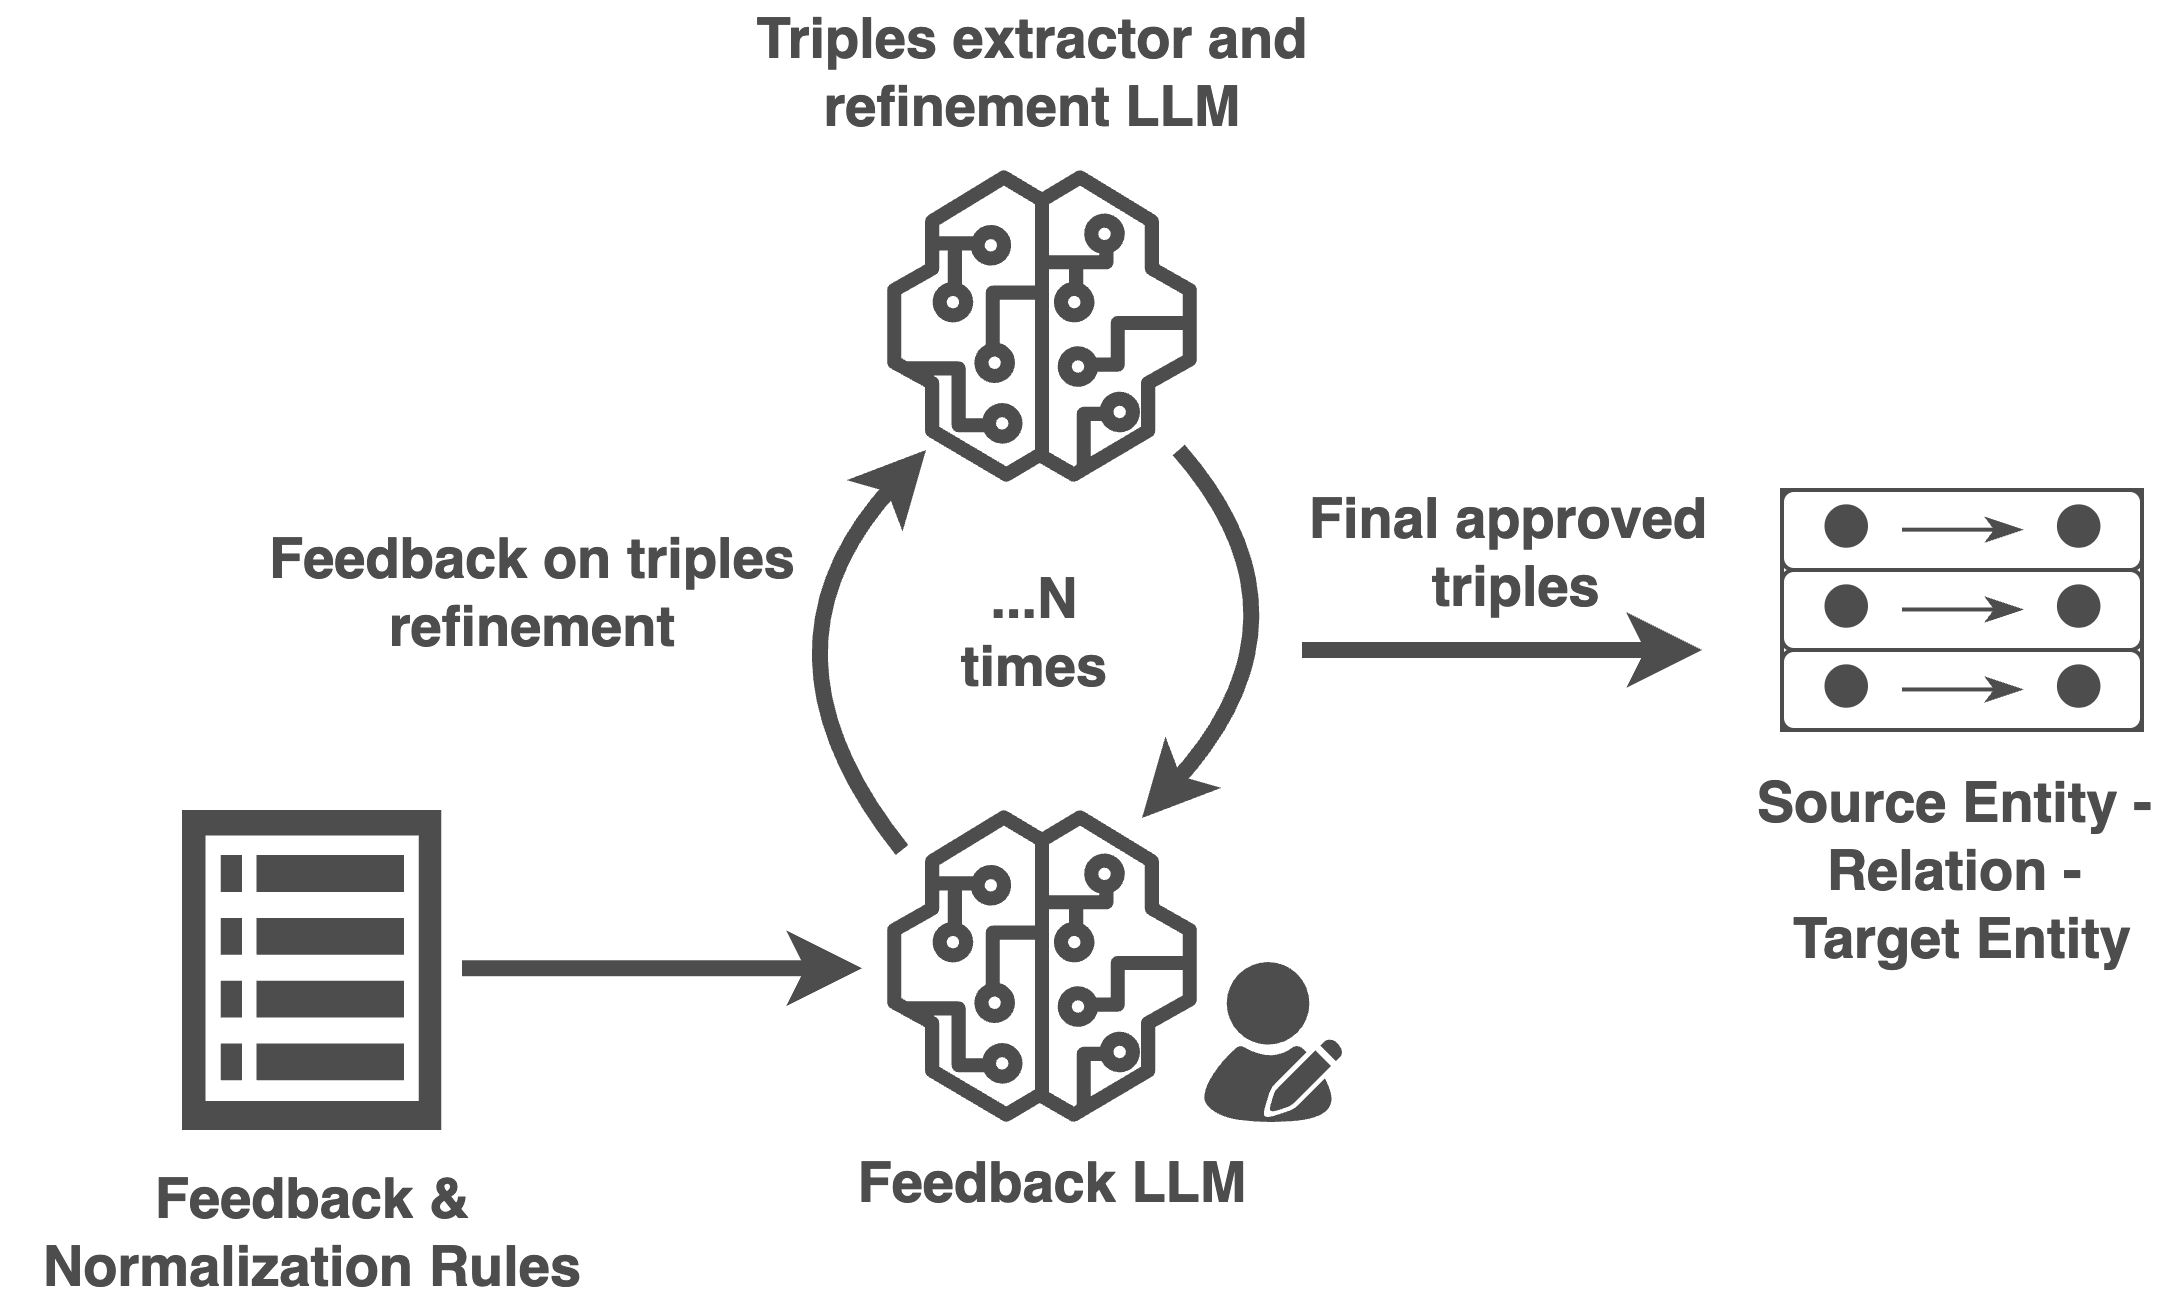
\includegraphics[width=\columnwidth]{figures/reflection_diagram.png}
    \caption{Overview of Reflection Agent where the triples are refined using an iterative feedback loop}
    \label{fig:reflection_paradigm}
\end{figure}

This iterative prompt engineering \& agentic approach advances the current state of domain‐specific KG extraction and offers a reusable framework for other regulated domains.

